\documentclass[12pt,a4paper]{article}
\usepackage[utf8]{inputenc}
\usepackage[utf8]{vietnam}
\usepackage{graphicx}
\usepackage{listings}
\usepackage{xcolor}
\usepackage{hyperref}
\usepackage{geometry}
\usepackage{amsmath}
\usepackage{amssymb}
\usepackage{booktabs}
\usepackage{tikz}
\usetikzlibrary{shapes.geometric, arrows, positioning, trees}

\geometry{margin=1in}

\definecolor{codegreen}{rgb}{0,0.6,0}
\definecolor{codegray}{rgb}{0.5,0.5,0.5}
\definecolor{codepurple}{rgb}{0.58,0,0.82}
\definecolor{backcolour}{rgb}{0.96,0.96,0.93}

\lstdefinestyle{mystyle}{
    backgroundcolor=\color{backcolour},   
    commentstyle=\color{codegreen},
    keywordstyle=\color{magenta},
    numberstyle=\tiny\color{codegray},
    stringstyle=\color{codepurple},
    basicstyle=\ttfamily\footnotesize,
    breakatwhitespace=false,         
    breaklines=true,                 
    captionpos=b,                    
    keepspaces=true,                 
    numbers=left,                    
    numbersep=5pt,                  
    showspaces=false,                
    showstringspaces=false,
    showtabs=false,                  
    tabsize=2,
    language=C++
}

\lstset{style={mystyle}}

\title{\textbf{CS202 Design Pattern Report: Interpreter Pattern}\\\large Formal Grammars, Abstract Syntax Trees, and Modern C++ Memory Architectures}
\author{\textbf{Group 52} \\ Nguyễn Đình Minh Huy (Student ID: 25125083) \\ Trần Gia Huy (Student ID: 25125084)}
\date{\today}

\begin{document}

\maketitle
\tableofcontents
\newpage

\section{Real-world Problem \& Theoretical Motivation}

\subsection{Background and Domain-Specific Languages (DSLs)}
In software engineering, systems frequently encounter requirements to interpret, evaluate, or execute statements written in domain-specific mini-languages at runtime. Unlike general-purpose programming languages (e.g., C++, Java, Rust), domain-specific languages (DSLs) are tailored to specialized problem domains. Prominent examples include:
\begin{itemize}
    \item \textbf{Dynamic Business Rule Engines:} Validating loan eligibility, risk scoring, or discount tiers defined by non-developer business analysts.
    \item \textbf{Database Query and Filter Parsers:} Evaluating SQL-like \texttt{WHERE} clauses (e.g., \texttt{age > 21 AND status == 'ACTIVE'}) dynamically generated from user search interfaces.
    \item \textbf{IoT Sensor Event Processing:} Filtering high-throughput telemetry streams against custom user-defined logic conditions (e.g., \texttt{temp > 85.0 OR (pressure > 120.0 AND NOT valve\_open)}).
    \item \textbf{Configuration-Driven Access Control (RBAC/ABAC):} Evaluating permission predicates such as \texttt{(isOwner OR isAdmin) AND NOT isBanned}.
\end{itemize}

Hardcoding every permutation of logical rules into static source code results in severe inflexibility. Every rule change requires recompilation, regression testing, and deployment. Consequently, systems require a mechanism to define, compose, and evaluate arbitrary sentences of a well-defined language dynamically at runtime.

\subsection{Problem Statement: Boolean Logic Evaluator}
To illustrate the problem concretely, consider a configurable logic engine that evaluates Boolean expressions consisting of:
\begin{enumerate}
    \item \textbf{Variables:} Identifiers representing dynamic state (e.g., $A, B, C$).
    \item \textbf{Constants:} Literal truth values (\texttt{true}, \texttt{false}).
    \item \textbf{Unary Operators:} Logical negation (\texttt{NOT} / $\neg$).
    \item \textbf{Binary Operators:} Conjunction (\texttt{AND} / $\land$), Disjunction (\texttt{OR} / $\lor$), and Exclusive-OR (\texttt{XOR} / $\oplus$).
    \item \textbf{Groupings:} Nested parentheses controlling operator precedence.
\end{enumerate}

The engine must take an expression along with a symbol table (a \textit{Context} mapping identifiers to their Boolean values) and compute the exact truth result according to standard mathematical logic.

\subsection{Language Grammar and Operator Rules}
To keep the design clear and practical, the language is defined by simple composition rules rather than formal compiler notation:
\begin{itemize}
    \item \textbf{Atomic Expressions (Terminals):} Either a named variable (e.g., $A, B$) looked up from the \texttt{Context} or a literal Boolean constant (\texttt{true}, \texttt{false}).
    \item \textbf{Unary Operation:} Negation (\texttt{NOT}) operating on a single child expression.
    \item \textbf{Binary Operations:} Conjunction (\texttt{AND}), Disjunction (\texttt{OR}), and Exclusive-OR (\texttt{XOR}) combining two child sub-expressions.
    \item \textbf{Operator Precedence:} Evaluated in standard algebraic order: $\text{NOT} > \text{AND} > \text{XOR} > \text{OR}$, with nested sub-expressions enclosed in parentheses evaluated first.
\end{itemize}

By organizing expressions according to these simple rules, any valid logical statement can be translated directly into a hierarchical tree structure.

\newpage
\section{Naive Solution (Without Design Pattern)}

In a naive C++ implementation, expressions are treated as raw text strings. The evaluation is performed through manual string searching, linear token splitting, or ad-hoc procedural loops.

\begin{lstlisting}[caption=Naive Boolean Expression Evaluator (\texttt{naive.cpp})]
// Context: Maps variable names to boolean values
class Context {
public:
    void assign(const std::string& name, bool value) { variables_[name] = value; }
    bool lookup(const std::string& name) const {
        auto it = variables_.find(name);
        if (it == variables_.end()) throw std::runtime_error("Unknown variable: " + name);
        return it->second;
    }
private:
    std::map<std::string, bool> variables_;
};

class NaiveLogicEvaluator {
public:
    // Evaluates flat left-to-right expressions (e.g. "A AND B OR C")
    static bool evaluate(const std::string& expression, const Context& context) {
        std::vector<std::string> tokens = tokenize(expression);
        if (tokens.empty()) return false;

        bool result = parseOperand(tokens[0], context);

        for (size_t i = 1; i + 1 < tokens.size(); i += 2) {
            const std::string& op = tokens[i];
            bool rhs = parseOperand(tokens[i + 1], context);

            if (op == "AND") {
                result = result && rhs;
            } else if (op == "OR") {
                result = result || rhs;
            } else if (op == "XOR") {
                result = result ^ rhs;
            } else {
                throw std::invalid_argument("Unsupported operator: " + op);
            }
        }
        return result;
    }

private:
    static bool parseOperand(const std::string& token, const Context& context) {
        if (token == "true" || token == "1") return true;
        if (token == "false" || token == "0") return false;
        return context.lookup(token);
    }

    static std::vector<std::string> tokenize(const std::string& expression) {
        std::stringstream ss(expression);
        std::string token;
        std::vector<std::string> tokens;
        while (ss >> token) tokens.push_back(token);
        return tokens;
    }
};
\end{lstlisting}

\subsection{Step-by-Step Execution of the Naive Evaluator}
To illustrate how the naive solution operates, consider evaluating the string \texttt{"A OR B AND C"} with context $A=\text{true}, B=\text{false}, C=\text{true}$:
\begin{enumerate}
    \item \textbf{Tokenization (String Splitting):} The evaluator parses the raw string by whitespace into a linear token vector:
    \begin{equation*}
        \text{\texttt{tokens}} = \big[\text{"A"}, \; \text{"OR"}, \; \text{"B"}, \; \text{"AND"}, \; \text{"C"}\big]
    \end{equation*}
    \item \textbf{Initial Left Operand Lookup:} The first token \texttt{"A"} is looked up in \texttt{Context} ($A = \text{true}$) to initialize the running accumulator \texttt{result = true}.
    \item \textbf{Linear Left-to-Right Evaluation Loop:} The loop steps through consecutive operator-operand pairs:
    \begin{itemize}
        \item \textit{Step 3a:} Reads operator \texttt{"OR"} and operand \texttt{"B"} ($B = \text{false}$). Updates:
        \begin{equation*}
            \text{\texttt{result}} = \text{\texttt{result}} \lor B = \text{true} \lor \text{false} = \mathbf{true}
        \end{equation*}
        \item \textit{Step 3b:} Reads operator \texttt{"AND"} and operand \texttt{"C"} ($C = \text{true}$). Updates:
        \begin{equation*}
            \text{\texttt{result}} = \text{\texttt{result}} \land C = \text{true} \land \text{true} = \mathbf{true}
        \end{equation*}
    \end{itemize}
\end{enumerate}

\textbf{Critical Flaw Demonstrated:} The naive evaluator computes $(A \lor B) \land C = (\text{true} \lor \text{false}) \land \text{true} = \text{true}$. If the input were \texttt{"false OR true AND false"}, the mathematically correct precedence $A \lor (B \land C)$ yields $\text{false} \lor (\text{true} \land \text{false}) = \mathbf{false}$, but the naive left-to-right evaluator incorrectly outputs $(\text{false} \lor \text{true}) \land \text{false} = \mathbf{false}$ (or in other expressions, completely corrupts truth values due to lack of precedence and parenthesis support).

\newpage
\section{In-Depth Analysis of Naive Solution Drawbacks}

The naive string-scanning and procedural dispatch approach presents several architectural, correctness, and performance limitations:

\begin{table}[h]
\centering
\small
\begin{tabular}{p{3.8cm} p{5.5cm} p{5.5cm}}
\toprule
\textbf{Deficiency Area} & \textbf{Manifestation in Naive Code} & \textbf{Architectural Consequence} \\
\midrule
\textbf{Open-Closed Principle (OCP) Violation} & Adding an operator (e.g., \texttt{NAND}, \texttt{IMPLIES}) requires modifying the central \texttt{if-else} loop in \texttt{evaluate()}. & Existing evaluation code must be modified, increasing regression risk. \\
\addlinespace
\textbf{Single Responsibility Principle (SRP) Violation} & \texttt{NaiveLogicEvaluator} handles lexical tokenization, semantic validation, operator precedence, and evaluation in one class. & Parsing and evaluation logic cannot be tested or maintained independently. \\
\addlinespace
\textbf{Operator Precedence Limitations} & Evaluates flat expressions strictly left-to-right. \texttt{A OR B AND C} evaluates as $(A \lor B) \land C$ instead of $A \lor (B \land C)$. & Produces incorrect results for expressions requiring operator precedence. \\
\addlinespace
\textbf{Nesting and Parentheses Support} & Supporting nested sub-expressions (e.g., \texttt{(A AND (NOT B)) OR C}) requires recursive regex or complex stack tracking. & Significantly increases procedural string manipulation complexity. \\
\addlinespace
\textbf{Evaluation Overhead} & String allocations, repeated \texttt{substr()} calls, and linear scans incur additional overhead on repeated evaluations. & Inefficient when expressions are evaluated repeatedly against changing contexts. \\
\bottomrule
\end{tabular}
\caption{Design and Performance Limitations of the Naive Solution}
\end{table}

\section{Introduction to the Interpreter Design Pattern}

\subsection{Definition and Intent}
According to the Gang of Four (GoF), the \textbf{Interpreter Pattern} is defined as:
\begin{quote}
\textit{"Given a language, define a representation for its grammar along with an interpreter that uses the representation to interpret sentences in the language."}
\end{quote}

The pattern addresses the problem by representing each grammar rule as a class. The syntax of an expression is represented as an \textbf{Abstract Syntax Tree (AST)}, where each node is an instance of an expression class. Evaluation is performed by traversing the tree recursively.

\subsection{Key Structural Components}
\begin{itemize}
    \item \textbf{Context (\texttt{Context}):} Encapsulates the global execution environment, maintaining state such as variable bindings (symbol table) needed by terminal expressions.
    \item \textbf{AbstractExpression (\texttt{BooleanExpression}):} Declares an abstract interface with an evaluation method:
    \begin{equation*}
        \text{\texttt{virtual bool interpret(const Context\& context) const = 0;}}
    \end{equation*}
    \item \textbf{TerminalExpression (\texttt{VariableExpression}, \texttt{ConstantExpression}):} Represents leaf nodes corresponding to terminal grammar symbols. Directly evaluates based on the provided \texttt{Context}.
    \item \textbf{NonterminalExpression (\texttt{AndExpression}, \texttt{OrExpression}, \texttt{NotExpression}, \texttt{XorExpression}):} Represents internal nodes of the AST corresponding to grammar production rules. Contains child \texttt{AbstractExpression} instances and aggregates their recursive evaluations.
    \item \textbf{Client:} Assembles (or receives from a parser) the composite AST hierarchy and initiates evaluation by invoking \texttt{interpret()} on the root node.
\end{itemize}


\newpage
\section{UML Class Diagrams}

\subsection{General GoF Interpreter Pattern Structure}
The Interpreter pattern defines a polymorphic hierarchy where non-terminal composite nodes hold references to abstract expressions, while terminal nodes evaluate directly against the context.

\begin{figure}[htbp]
\centering
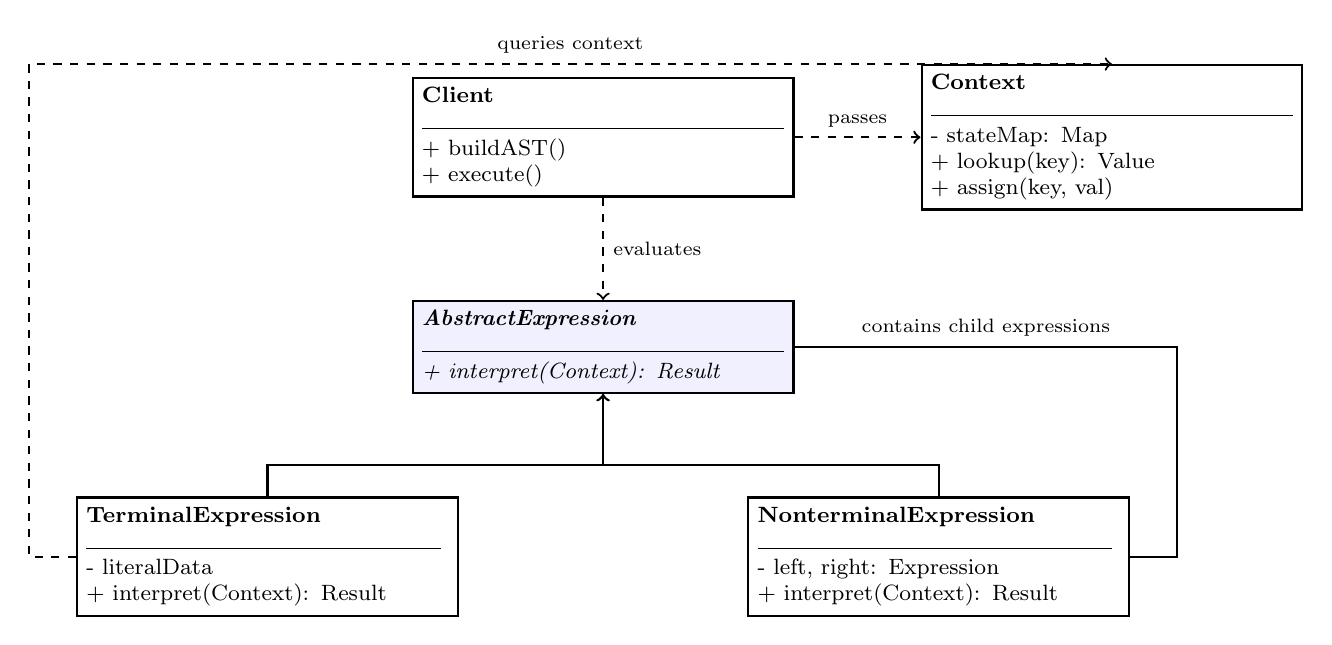
\begin{tikzpicture}[
    class/.style={rectangle, draw=black, thick, fill=white, text width=4.6cm, minimum height=1.0cm, font=\footnotesize},
    abstract/.style={class, fill=blue!6}
]
\node[class] (client) {\textbf{Client}\\\rule{4.6cm}{0.3pt}\\+ buildAST()\\+ execute()};
\node[class, right=1.6cm of client] (context) {\textbf{Context}\\\rule{4.6cm}{0.3pt}\\- stateMap: Map\\+ lookup(key): Value\\+ assign(key, val)};
\node[abstract, below=1.3cm of client] (abstractExp) {\textbf{\textit{AbstractExpression}}\\\rule{4.6cm}{0.3pt}\\\textit{+ interpret(Context): Result}};

\node[class, below left=1.3cm and -0.6cm of abstractExp] (terminal) {\textbf{TerminalExpression}\\\rule{4.5cm}{0.3pt}\\- literalData\\+ interpret(Context): Result};
\node[class, below right=1.3cm and -0.6cm of abstractExp] (nonterminal) {\textbf{NonterminalExpression}\\\rule{4.5cm}{0.3pt}\\- left, right: Expression\\+ interpret(Context): Result};

\draw[->, thick, dashed] (client) -- (abstractExp) node[midway, right, font=\scriptsize] {evaluates};
\draw[->, thick, dashed] (client) -- (context) node[midway, above, font=\scriptsize] {passes};

% Route terminal queries context cleanly around the perimeter to avoid intersecting AbstractExpression
\draw[->, thick, dashed] (terminal.west) -- ++(-0.6,0) |- (context.north) node[near end, above, font=\scriptsize] {queries context};

\draw[->, thick] (terminal.north) -- ++(0,0.4) -| (abstractExp.south);
\draw[->, thick] (nonterminal.north) -- ++(0,0.4) -| (abstractExp.south);
\draw[thick] (nonterminal.east) -- ++(0.6,0) |- (abstractExp.east) node[near end, above, font=\scriptsize] {contains child expressions};
\end{tikzpicture}
\caption{General GoF Interpreter Pattern UML Structure}
\label{fig:general_uml_structure}
\end{figure}

\subsection{Boolean Logic Evaluator Class Hierarchy}
For our Boolean expression engine, \texttt{BooleanExpression} acts as the abstract component interface with concrete terminals (\texttt{VariableExpression}, \texttt{ConstantExpression}) and non-terminals owning child expressions via \texttt{std::unique\_ptr}.

\begin{figure}[htbp]
\centering
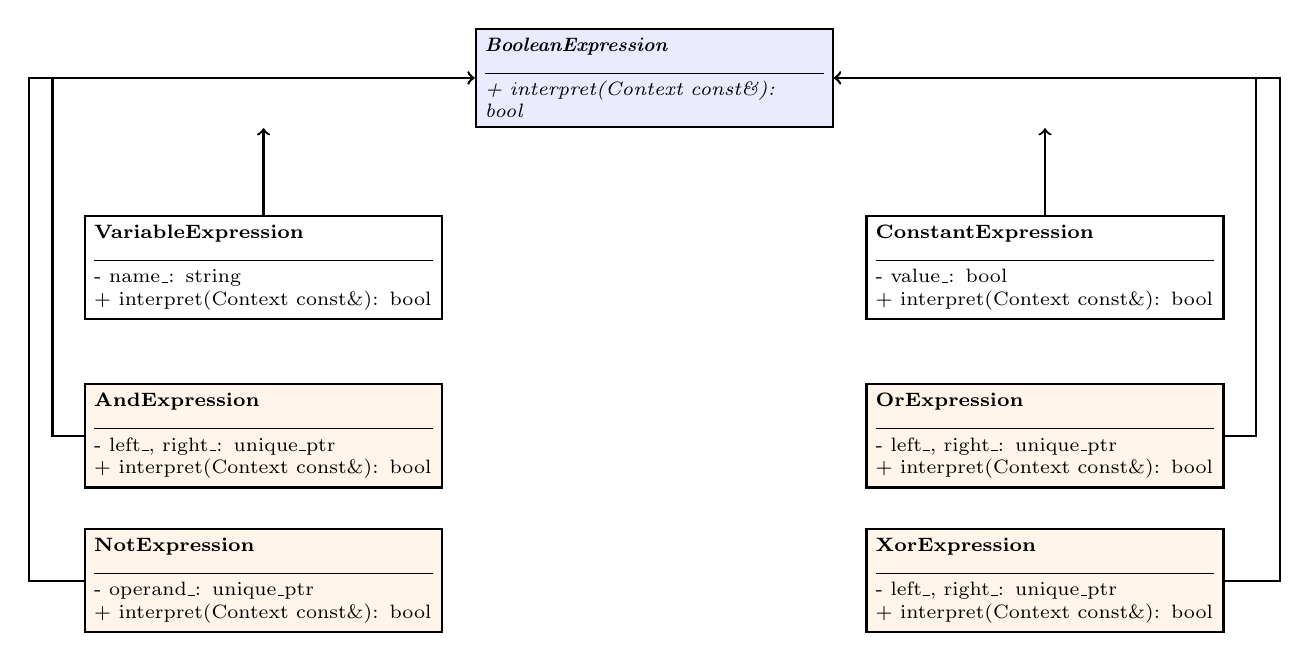
\begin{tikzpicture}[
    class/.style={rectangle, draw=black, thick, fill=white, text width=4.3cm, font=\scriptsize},
    abstract/.style={class, fill=blue!8},
    opclass/.style={class, fill=orange!8}
]
\node[abstract] (exp) {\textbf{\textit{BooleanExpression}}\\\rule{4.3cm}{0.3pt}\\\textit{+ interpret(Context const\&): bool}};

\node[class, below left=1.1cm and 0.4cm of exp] (varExp) {\textbf{VariableExpression}\\\rule{4.3cm}{0.3pt}\\- name\_: string\\+ interpret(Context const\&): bool};
\node[class, below right=1.1cm and 0.4cm of exp] (constExp) {\textbf{ConstantExpression}\\\rule{4.3cm}{0.3pt}\\- value\_: bool\\+ interpret(Context const\&): bool};

\node[opclass, below=0.8cm of varExp] (andExp) {\textbf{AndExpression}\\\rule{4.3cm}{0.3pt}\\- left\_, right\_: unique\_ptr\\+ interpret(Context const\&): bool};
\node[opclass, below=0.8cm of constExp] (orExp) {\textbf{OrExpression}\\\rule{4.3cm}{0.3pt}\\- left\_, right\_: unique\_ptr\\+ interpret(Context const\&): bool};

\node[opclass, below=0.5cm of andExp] (notExp) {\textbf{NotExpression}\\\rule{4.3cm}{0.3pt}\\- operand\_: unique\_ptr\\+ interpret(Context const\&): bool};
\node[opclass, below=0.5cm of orExp] (xorExp) {\textbf{XorExpression}\\\rule{4.3cm}{0.3pt}\\- left\_, right\_: unique\_ptr\\+ interpret(Context const\&): bool};

% Clean orthogonal inheritance lines directly to BooleanExpression
\draw[->, thick] (varExp.north) -- (varExp.north |- exp.south);
\draw[->, thick] (constExp.north) -- (constExp.north |- exp.south);

\draw[->, thick] (andExp.west) -- ++(-0.4,0) |- (exp.west);
\draw[->, thick] (notExp.west) -- ++(-0.7,0) |- (exp.west);

\draw[->, thick] (orExp.east) -- ++(0.4,0) |- (exp.east);
\draw[->, thick] (xorExp.east) -- ++(0.7,0) |- (exp.east);
\end{tikzpicture}
\caption{Concrete Boolean Logic Evaluator Class Hierarchy}
\label{fig:concrete_uml}
\end{figure}

\newpage
\section{Pattern-Based Implementation in C++17}

\subsection{Architectural Design Rationale: Strict AST vs. ASG/DAG}
A key design decision in our C++ implementation is enforcing a strict \textbf{Abstract Syntax Tree (AST)} rather than an \textbf{Abstract Semantic Graph (ASG / DAG)}:
\begin{itemize}
    \item \textbf{Strict Tree Structure (\texttt{std::unique\_ptr}):} Every expression node has exactly \textit{one unique parent}. Duplicate occurrences of a variable (such as $A$ appearing in multiple sub-clauses) are instantiated as distinct terminal leaves. This is enforced using \texttt{std::unique\_ptr} with move semantics, eliminating reference counting overhead and ensuring deterministic single-owner memory reclamation.
    \item \textbf{Graph Alternative (\texttt{std::shared\_ptr}):} In optimizing engines with Common Subexpression Elimination (CSE), identical sub-expressions share node instances with multiple parents (a DAG). However, this introduces atomic reference counting overhead and cache complexity.
\end{itemize}

\subsection{Source Code Implementation}
The following listings demonstrate the complete, robust implementation using C++17 move semantics and unique pointers (\texttt{Interpreter/src/pattern.cpp}).

\begin{lstlisting}[caption=Context and Abstract Expression Interface]
#include <iostream>
#include <string>
#include <map>
#include <memory>
#include <stdexcept>

namespace pattern {

// Context: Holds runtime symbol bindings
class Context {
public:
    void assign(const std::string& name, bool value) {
        variables_[name] = value;
    }

    bool lookup(const std::string& name) const {
        auto it = variables_.find(name);
        if (it == variables_.end()) {
            throw std::runtime_error("Unbound variable in Context: " + name);
        }
        return it->second;
    }

private:
    std::map<std::string, bool> variables_;
};

// Abstract Expression Interface
class BooleanExpression {
public:
    virtual ~BooleanExpression() = default;
    virtual bool interpret(const Context& context) const = 0;
};
\end{lstlisting}

\begin{lstlisting}[caption=Terminal Expressions: Variables and Constants]
// Terminal Expression: Variable Lookup
class VariableExpression : public BooleanExpression {
public:
    explicit VariableExpression(std::string name) : name_(std::move(name)) {}

    bool interpret(const Context& context) const override {
        return context.lookup(name_);
    }

private:
    std::string name_;
};

// Terminal Expression: Boolean Literal Constant
class ConstantExpression : public BooleanExpression {
public:
    explicit ConstantExpression(bool value) : value_(value) {}

    bool interpret(const Context&) const override {
        return value_;
    }

private:
    bool value_;
};
\end{lstlisting}

\newpage
\begin{lstlisting}[caption={Non-Terminal Expressions: AND, OR, NOT, XOR with Unique Ownership}]
// Non-Terminal: Logical Conjunction (AND)
class AndExpression : public BooleanExpression {
public:
    AndExpression(std::unique_ptr<BooleanExpression> left, std::unique_ptr<BooleanExpression> right)
        : left_(std::move(left)), right_(std::move(right)) {}

    bool interpret(const Context& context) const override {
        return left_->interpret(context) && right_->interpret(context);
    }

private:
    std::unique_ptr<BooleanExpression> left_;
    std::unique_ptr<BooleanExpression> right_;
};

// Non-Terminal: Logical Disjunction (OR)
class OrExpression : public BooleanExpression {
public:
    OrExpression(std::unique_ptr<BooleanExpression> left, std::unique_ptr<BooleanExpression> right)
        : left_(std::move(left)), right_(std::move(right)) {}

    bool interpret(const Context& context) const override {
        return left_->interpret(context) || right_->interpret(context);
    }

private:
    std::unique_ptr<BooleanExpression> left_;
    std::unique_ptr<BooleanExpression> right_;
};

// Non-Terminal: Logical Negation (NOT)
class NotExpression : public BooleanExpression {
public:
    explicit NotExpression(std::unique_ptr<BooleanExpression> operand)
        : operand_(std::move(operand)) {}

    bool interpret(const Context& context) const override {
        return !operand_->interpret(context);
    }

private:
    std::unique_ptr<BooleanExpression> operand_;
};

// Non-Terminal: Exclusive-OR (XOR)
class XorExpression : public BooleanExpression {
public:
    XorExpression(std::unique_ptr<BooleanExpression> left, std::unique_ptr<BooleanExpression> right)
        : left_(std::move(left)), right_(std::move(right)) {}

    bool interpret(const Context& context) const override {
        return left_->interpret(context) ^ right_->interpret(context);
    }

private:
    std::unique_ptr<BooleanExpression> left_;
    std::unique_ptr<BooleanExpression> right_;
};

} // namespace pattern
\end{lstlisting}

\newpage
\subsection{Execution Walkthrough \& Step-by-Step AST Evaluation Trace}

Consider the composite logical expression:
\begin{equation}
\text{Expression} = (A \land (\neg B)) \lor (C \oplus A)
\end{equation}
Given the runtime variable bindings in Context:
\begin{equation*}
A = \mathbf{true}, \quad B = \mathbf{false}, \quad C = \mathbf{true}
\end{equation*}

\begin{lstlisting}[caption=Building and Evaluating the AST]
void runPatternDemo() {
    pattern::Context context;
    context.assign("A", true);
    context.assign("B", false);
    context.assign("C", true);

    // Build AST: (A AND (NOT B)) OR (C XOR A)
    auto notB = std::make_unique<pattern::NotExpression>(
        std::make_unique<pattern::VariableExpression>("B")
    );
    auto aAndNotB = std::make_unique<pattern::AndExpression>(
        std::make_unique<pattern::VariableExpression>("A"),
        std::move(notB)
    );
    auto cXorA = std::make_unique<pattern::XorExpression>(
        std::make_unique<pattern::VariableExpression>("C"),
        std::make_unique<pattern::VariableExpression>("A")
    );
    auto fullExpr = std::make_unique<pattern::OrExpression>(
        std::move(aAndNotB),
        std::move(cXorA)
    );

    bool result = fullExpr->interpret(context);
    std::cout << "Result: " << (result ? "true" : "false") << "\n"; // Outputs: true
}
\end{lstlisting}

\subsubsection{Step-by-Step Recursive Trace Table}
During the post-order depth-first traversal of the AST, the nodes are evaluated in the following sequence:

\begin{table}[htbp]
\centering
\small
\begin{tabular}{c p{4.2cm} c c p{4.5cm}}
\toprule
\textbf{Step} & \textbf{Node Evaluated} & \textbf{Subtree} & \textbf{Value} & \textbf{Explanation / Operation} \\
\midrule
1 & \texttt{VariableExpression("B")} & $B$ & $\mathbf{false}$ & Context lookup returns $B = \text{false}$. \\
2 & \texttt{NotExpression} & $\neg B$ & $\mathbf{true}$ & Negation: $!\text{false} = \text{true}$. \\
3 & \texttt{VariableExpression("A")} & $A$ & $\mathbf{true}$ & Context lookup returns $A = \text{true}$. \\
4 & \texttt{AndExpression} & $A \land (\neg B)$ & $\mathbf{true}$ & Conjunction: $\text{true} \land \text{true} = \text{true}$. \\
5 & \texttt{VariableExpression("C")} & $C$ & $\mathbf{true}$ & Context lookup returns $C = \text{true}$. \\
6 & \texttt{VariableExpression("A")} & $A$ & $\mathbf{true}$ & Context lookup returns $A = \text{true}$. \\
7 & \texttt{XorExpression} & $C \oplus A$ & $\mathbf{false}$ & Exclusive OR: $\text{true} \oplus \text{true} = \text{false}$. \\
8 & \texttt{OrExpression} (Root) & $(A \land \neg B) \lor (C \oplus A)$ & $\mathbf{true}$ & Root Disjunction: $\text{true} \lor \text{false} = \mathbf{true}$. \\
\bottomrule
\end{tabular}
\caption{Recursive Post-Order Traversal Trace for AST Evaluation}
\end{table}

\newpage
\section{Evaluation of Trade-offs (Pros and Cons)}

\subsection{Advantages}
\begin{itemize}
    \item \textbf{High Grammar Extensibility (OCP Compliance):} Introducing new language constructs or operators (e.g., adding an \texttt{ImpliesExpression} for $P \implies Q \equiv \neg P \lor Q$) requires creating a new subclass of \texttt{BooleanExpression} without altering any existing classes.
    \item \textbf{Single Responsibility Principle (SRP):} Each class is strictly responsible for interpreting exactly one grammar symbol.
    \item \textbf{Decoupled Syntax Structure from Execution:} The structural representation (AST) is cleanly separated from the runtime evaluation state (\texttt{Context}).
    \item \textbf{Zero Evaluation Overhead with \texttt{std::unique\_ptr}:} By relying on direct polymorphic virtual dispatch and unique pointers, tree evaluation avoids string-slicing allocations and runs at native CPU speed.
\end{itemize}

\subsection{Disadvantages and Limitations}
\begin{itemize}
    \item \textbf{Combinatorial Class Explosion for Large Grammars:} For complex programming languages with hundreds of grammar production rules (e.g., full ECMAScript or SQL-92), maintaining hundreds of distinct AST classes manually becomes unmanageable.
    \item \textbf{Call-Stack Depth and Recursion Overhead:} Deeply nested syntax trees can lead to stack overflow if evaluated via naive recursion on resource-constrained embedded systems.
    \item \textbf{Grammar Maintenance Overhead:} Modifying operator precedence rules requires structural modifications to the AST assembly rather than simple configuration changes.
\end{itemize}

\section{Modern Web and Mobile Engineering Applications}

\subsection{Web Development Applications}
\begin{itemize}
    \item \textbf{Dynamic URL Routing Engines:} Modern web frameworks (e.g., Express.js, Fastify, React Router) translate parameterized route patterns (e.g., \texttt{/api/v1/users/:id/orders/:orderId}) into regex/AST matchers that extract path parameters from incoming HTTP request strings.
    \item \textbf{CSS Selector Engines:} Browser engines (e.g., WebKit, Blink) parse complex compound CSS selectors (e.g., \texttt{div.container > article:first-child p.lead}) into selector ASTs to efficiently match DOM nodes during style resolution.
    \item \textbf{Client-Side Formula Parsers:} Web spreadsheet applications (e.g., Google Sheets, Luckysheet) parse formula expressions (e.g., \texttt{=SUM(A1:A10) * IF(B1 > 50, 1.1, 1.0)}) into syntax trees that re-evaluate reactively upon cell updates.
\end{itemize}

\subsection{Mobile Development Applications}
\begin{itemize}
    \item \textbf{ICU MessageFormat \& Pluralization Parsers:} Mobile operating systems (iOS and Android) interpret dynamic localization strings containing gender, cardinal numbers, and pluralization branches (e.g., \texttt{"\{count, plural, =0\{No items\} =1\{One item\} other\{\# items\}\}"}).
    \item \textbf{Server-Driven UI (SDUI) Conditional Rendering:} Applications driven by backend layout schemas interpret JSON condition trees (e.g., \texttt{\{"and": [\{"user.isVip": true\}, \{"device.osVersion": "> 14"\}]\}}) to dynamically show or hide mobile screen widgets.
\end{itemize}

\newpage
\section{Advanced Architectural Combinations: Observer and Mediator Integration}

In real-world software architectures, design patterns rarely exist in isolation. The Interpreter pattern naturally combines with the **Observer** and **Mediator** patterns to create reactive, event-driven, and highly decoupled systems.

\subsection{Combining Interpreter with the Observer Pattern: Reactive Logic Evaluation}
In a static Interpreter implementation, clients must manually invoke \texttt{interpret()} whenever variable values change. In modern reactive architectures (such as reactive UI frameworks, spreadsheet dependency graphs, or IoT sensor triggers), this is refactored by applying the \textbf{Observer Pattern}:
\begin{itemize}
    \item \textbf{Reactive Context as Subject:} The \texttt{Context} acts as an observable \textit{Subject}. When a variable's value is modified via \texttt{Context::assign("temperature", 92.5)}, the Context publishes a state-change notification.
    \item \textbf{AST Roots as Observers:} Root expressions (or dependent UI components) register as \textit{Observers} listening to specific variable keys. Upon receiving an update event, they automatically trigger re-interpretation of their AST and emit new evaluation results reactively.
    \item \textbf{Benefit:} Eliminates wasteful CPU polling loops and enables push-based reactive logic engines.
\end{itemize}

\subsection{Combining Interpreter with the Mediator Pattern: Decoupled Command Coordination}
In complex distributed or multi-component systems (such as Air Traffic Control towers, CQRS command routers, or chat bot dispatchers), colleagues must coordinate without direct peer-to-peer coupling. Here, the \textbf{Mediator Pattern} leverages an internal \textbf{Interpreter}:
\begin{itemize}
    \item \textbf{Decoupled Colleague Interaction:} Colleague components (e.g., flights, sensor nodes, UI widgets) do not know about each other. Instead, they send declarative request/query sentences to a central \texttt{Mediator}.
    \item \textbf{Mediator as Rule Engine:} The central Mediator embeds an \texttt{Interpreter} engine to dynamically parse incoming command expressions, evaluate business rules, and check permission predicates before routing actions to target colleagues.
    \item \textbf{Benefit:} Completely decouples the communication topology ($O(N)$ star topology instead of $O(N^2)$ mesh) while retaining full flexibility to dynamically change business coordination rules at runtime.
\end{itemize}

\section{Conclusion}
The Interpreter Design Pattern provides an elegant, object-oriented solution for representing and evaluating dynamic domain-specific grammars. By modeling production rules as distinct classes and organizing them into an Abstract Syntax Tree (AST), the pattern achieves strict adherence to the Open-Closed and Single Responsibility Principles. 

Furthermore, combining the Interpreter pattern with modern C++17 memory management idioms—specifically using \textbf{\texttt{std::unique\_ptr}} for exclusive node ownership and zero-overhead move semantics—yields a high-performance, memory-safe execution engine. When combined with the Observer and Mediator patterns, it forms the backbone for reactive rule engines and decoupled, dynamic event-driven architectures.

\newpage

\section*{References}
\addcontentsline{toc}{section}{References}
\begin{itemize}
    \item Gamma, E., Helm, R., Johnson, R., \& Vlissides, J. (1994). \textit{Design Patterns: Elements of Reusable Object-Oriented Software}. Addison-Wesley.
    \item Aho, A. V., Lam, M. S., Sethi, R., \& Ullman, J. D. (2006). \textit{Compilers: Principles, Techniques, and Tools} (2nd ed.). Addison-Wesley.
    \item Meyers, S. (2014). \textit{Effective Modern C++: 42 Specific Ways to Improve Your Use of C++11 and C++14}. O'Reilly Media.
    \item Refactoring.Guru. \textit{Design Patterns: Interpreter Pattern}. \url{https://refactoring.guru/design-patterns/interpreter}
\end{itemize}

\end{document}

